\newpage
\chapter{PLANIFICACIÓN Y GESTIÓN DEL TFG}
\newpage

\newpage
\section{PLANIFICACIÓN DEL PROYECTO}

\subsection{Identificación de Interesados}
\begin{itemize}
\item \textbf{Usuarios de la aplicación web del museo}: Personas interesadas en la información ofrecida de las piezas expuestas en el museo que consultarán la página web.
\item \textbf{Tutor de este trabajo y administrador del museo}: Persona que ha propuesto el proyecto de digitalización del museo, y que lo administrará una vez terminado el desarrollo.
\item \textbf{Autora del trabajo y desarrolladora}: Encargada del desarrollo de la aplicación y de la documentación asociada.
\end{itemize}


\subsection{%OBS y 
PBS}
\begin{figure}[H]
\centering
\centerline{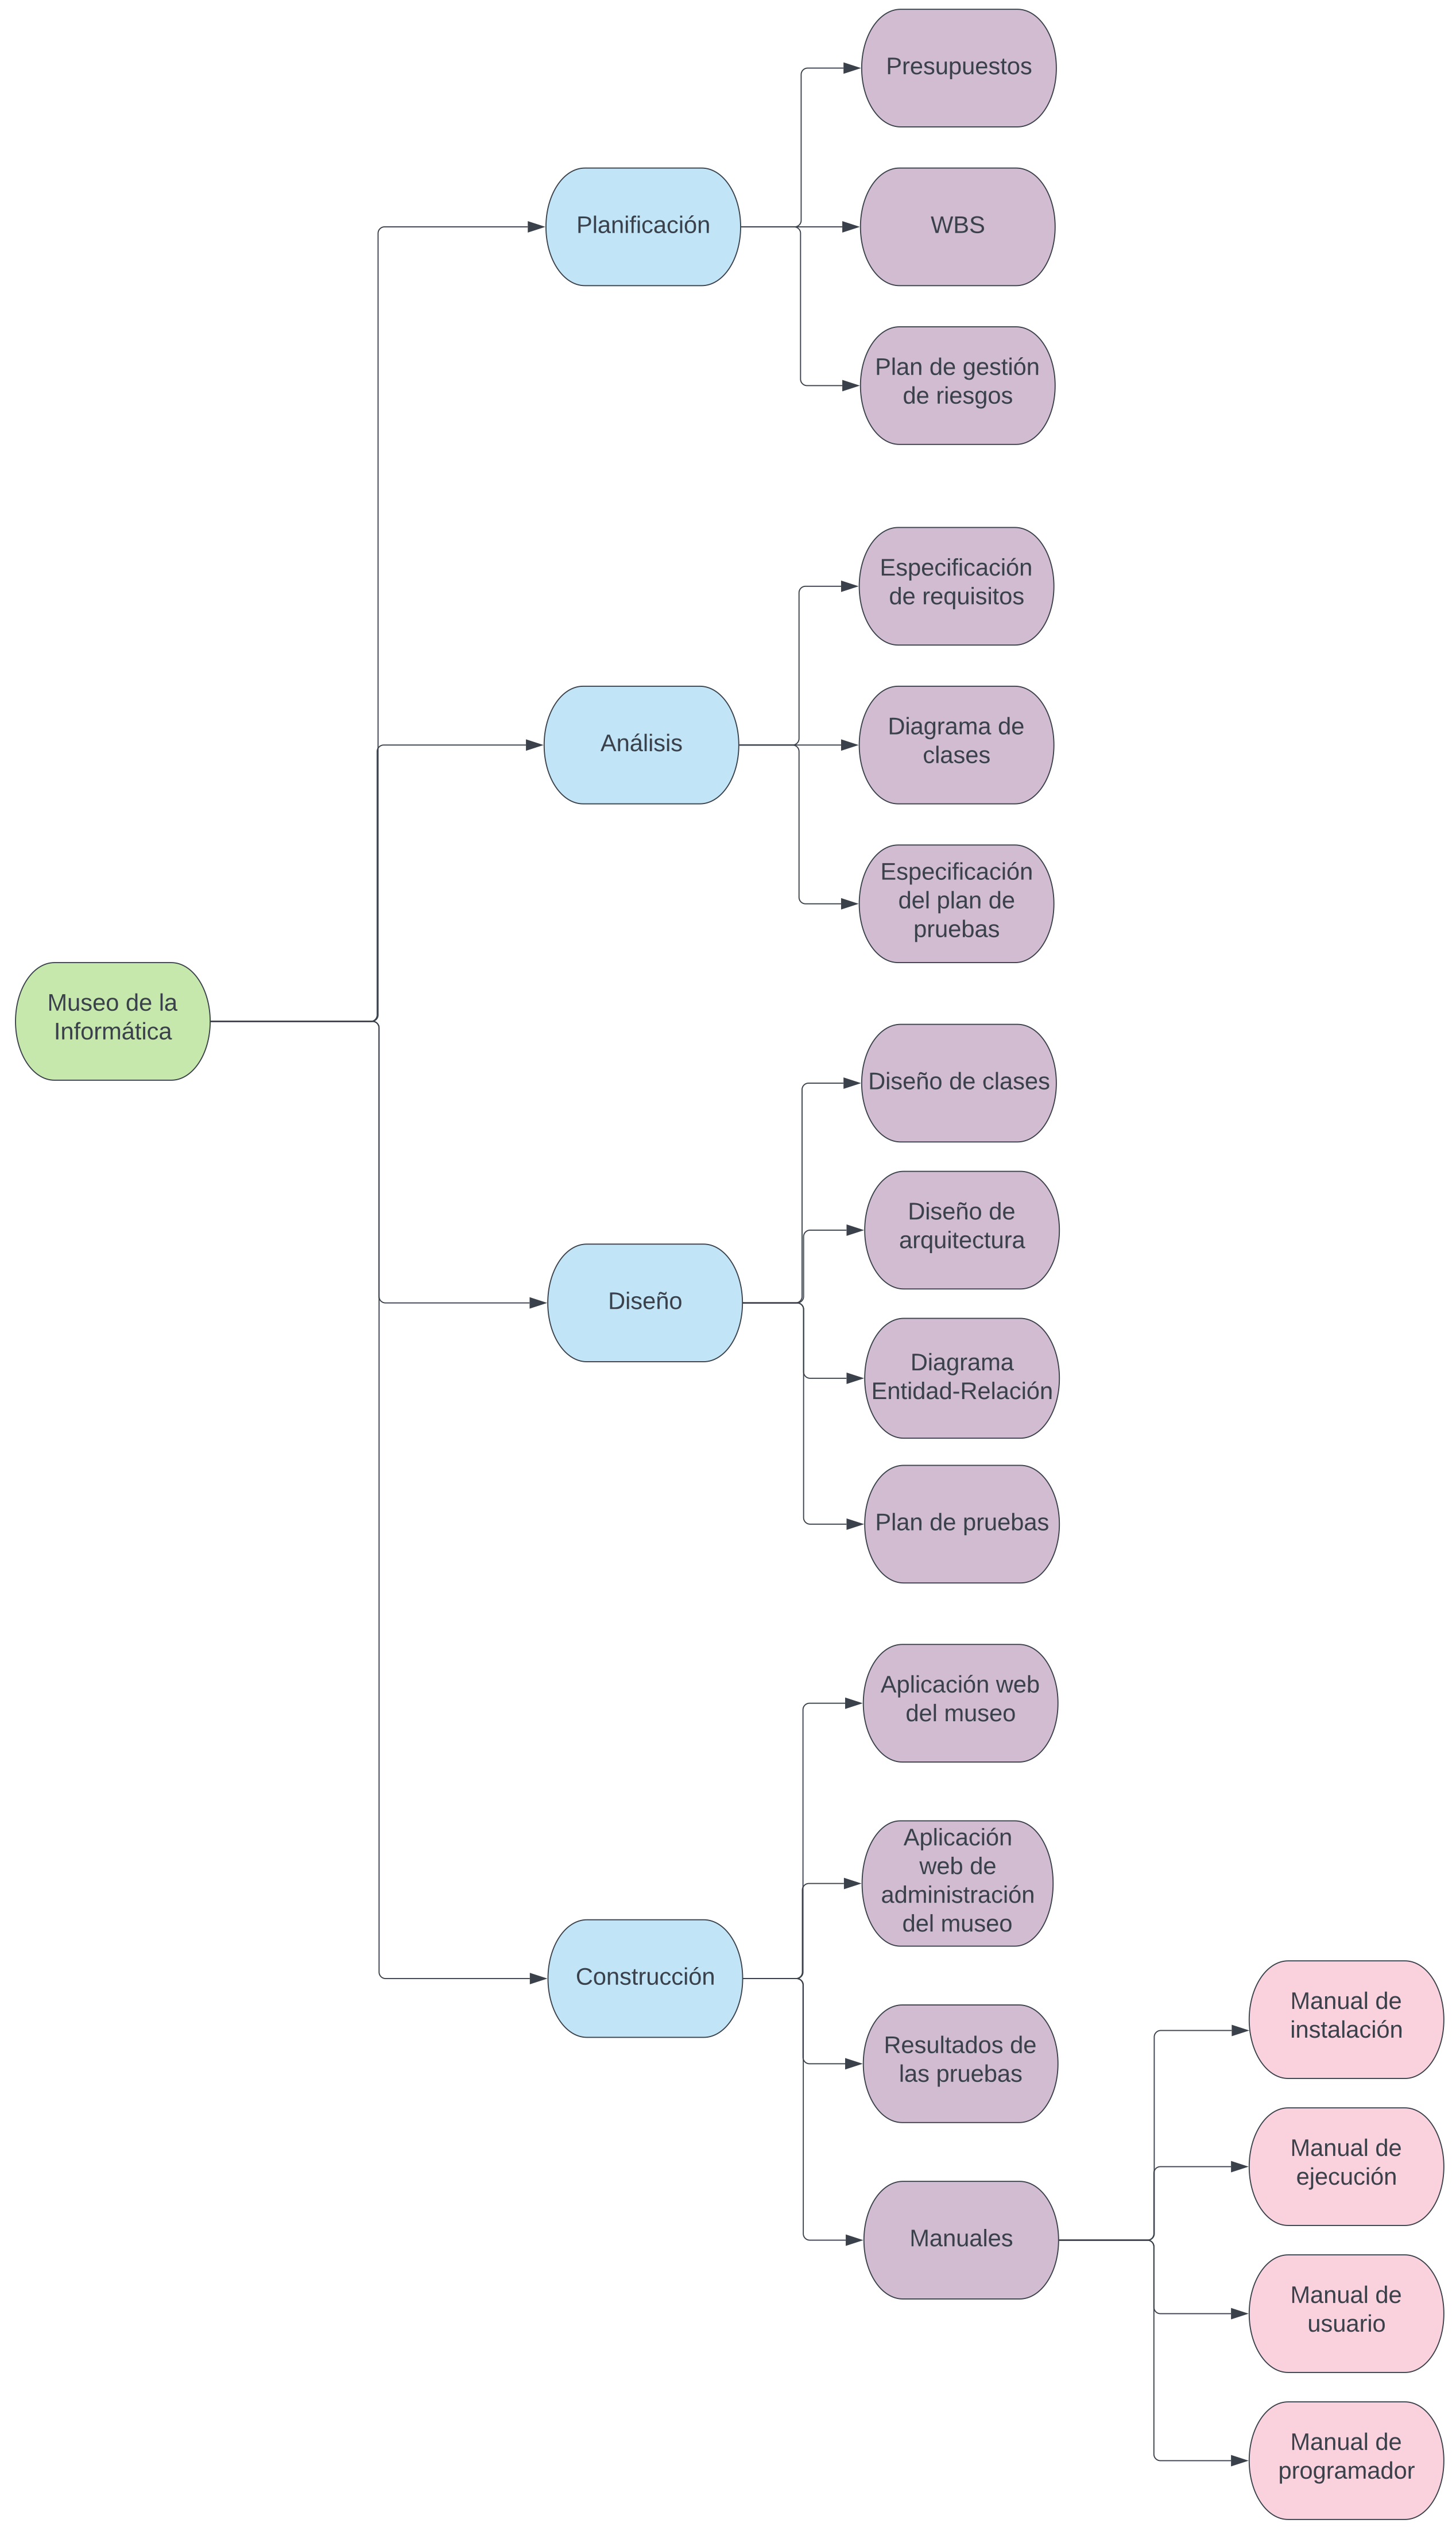
\includegraphics[scale=0.25]{PBS}}
\caption{Product Breakdown Structure}
\end{figure}


\subsection{Planificación Inicial. WBS}
A continuación se muestra la planificación inicial del proyecto y el correspondiente diagrama de Gantt. Para visualizar mejor esta planificación se adjunta el archivo \textit{WBS.mpp} como se especifica en la sección \ref{sec:contenido_anexos}. Se han planificado jornadas de trabajo de 3 horas diarias, y la estimación de la duración total del proyecto es de 258 horas.
\begin{landscape}
\pagestyle{empty}
\begin{figure}[H]
\centering
\centerline{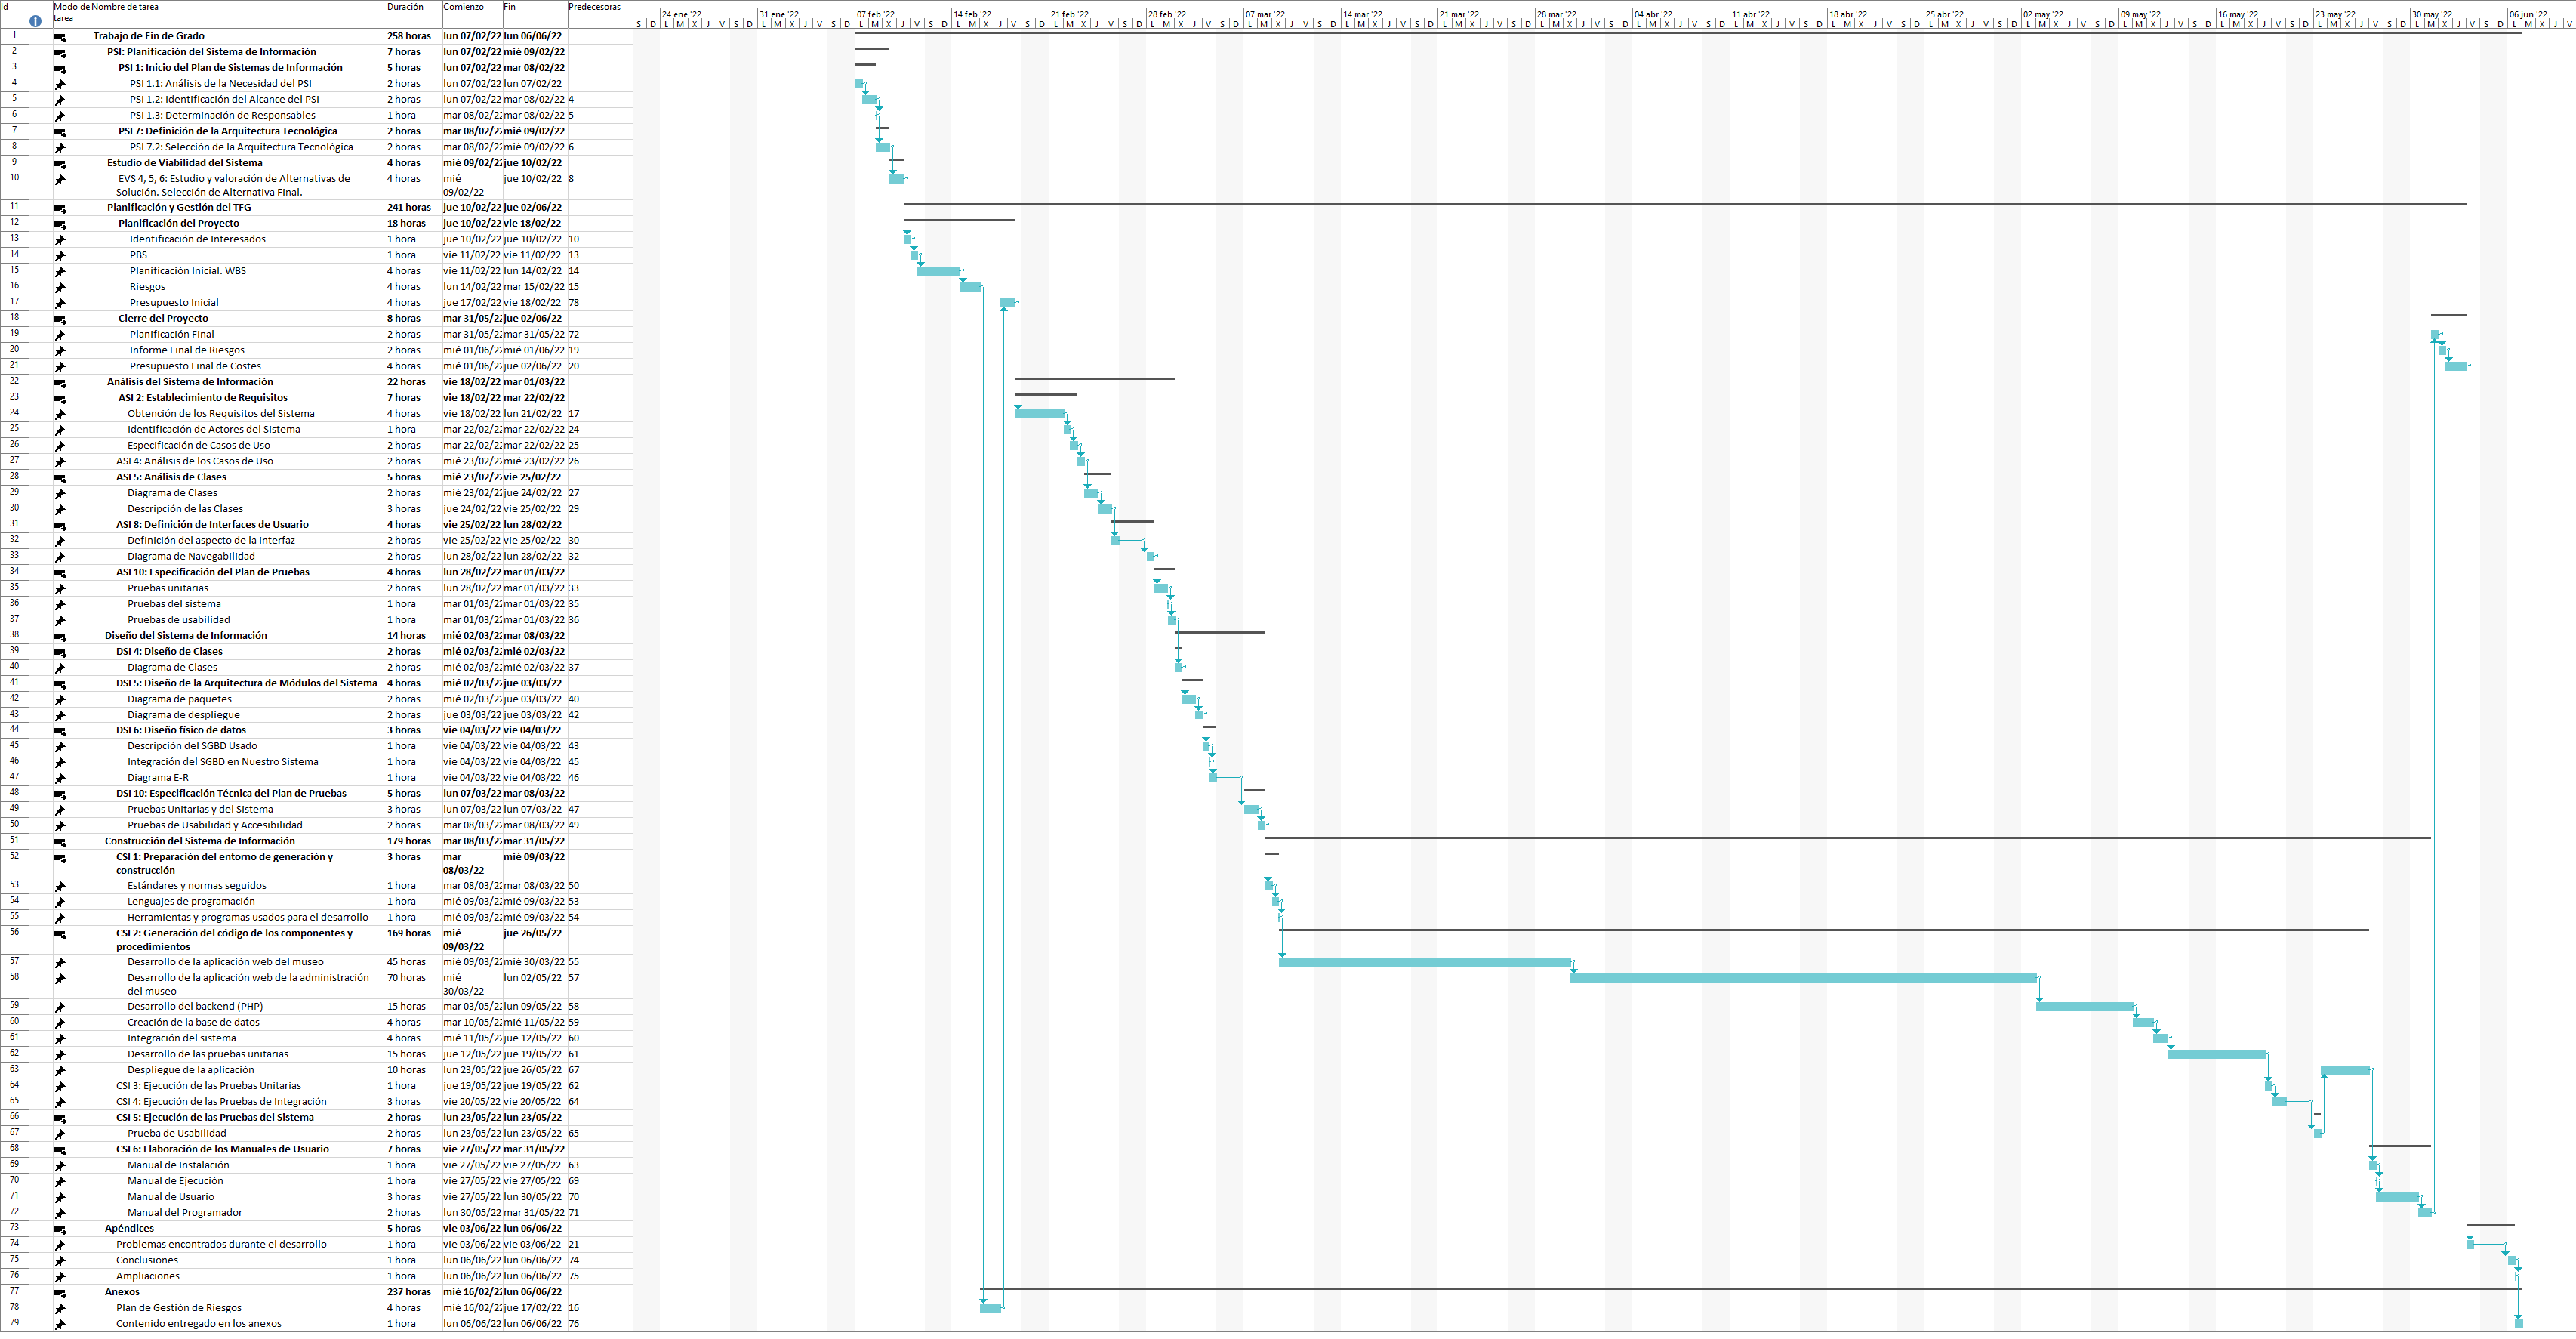
\includegraphics[scale=0.3]{plan-inicial}}
\caption{Planificación inicial, diagrama de Gantt}
\end{figure}

\end{landscape}
\pagestyle{fancy}
\subsection{Riesgos}\label{sec:riesgos}

\subsubsection{Plan de Gestión de Riesgos} 
El plan de gestión de riesgos del proyecto se define en el anexo \ref{sec:plan-riesgos}

\subsubsection{Identificación de Riesgos}

\subsubsection{Registro de Riesgos} 



\subsection{Presupuesto Inicial}

\subsubsection{Presupuesto de Costes}

\subsubsection{Presupuesto de Cliente} 


%\newpage
%\section{EJECUCIÓN DEL PROYECTO}
%
%\subsection{Plan Seguimiento de Planificación}
%
%\subsection{Bitácora de Incidencias del Proyecto}
%
%\subsection{Riesgos}


\newpage
\section{CIERRE DEL PROYECTO}

\subsection{Planificación Final}

\subsection{Informe Final de Riesgos}

\subsection{Presupuesto Final de Costes}

\subsection{Informe de Lecciones Aprendidas}
